For a system of two linear equations in the variables \(x,y\) what can our set of solutions look like?

Our set of solutions can appear as the intersection of two arbitrary lines. We essentially have three scenarios. The system can be represented by two non-parallel lines. In such case, there is one unique solution. The system can be represent by two parallel, distinct lines. In this case, there are no solutions. The third situation, each equation is represented by the exact same line. In this case, the lines are still considered parallel; however, they are not distinct. There are infinitely many solutions.

\begin{image}
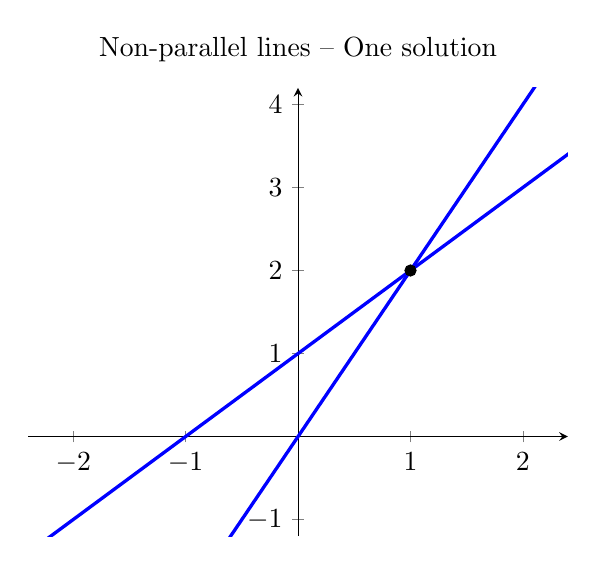
\begin{tikzpicture}
  \begin{axis}[
  title={Non-parallel lines -- One solution},
  xmin=-2.4,
  xmax=2.4,
  ymin=-1.2,
  ymax=4.2,
  axis lines=center,
  every axis y label/.style=
    {at=(current axis.above origin),anchor=south},
  every axis x label/.style=
    {at=(current axis.right of origin),anchor=west},
  ]
\addplot [very thick, blue, smooth, samples=100] {2*x};
\addplot [very thick, blue, smooth, samples=100] {x+1};
\addplot[mark=*] coordinates {(1,2)};
\end{axis}
\end{tikzpicture}
\end{image}
\begin{image}
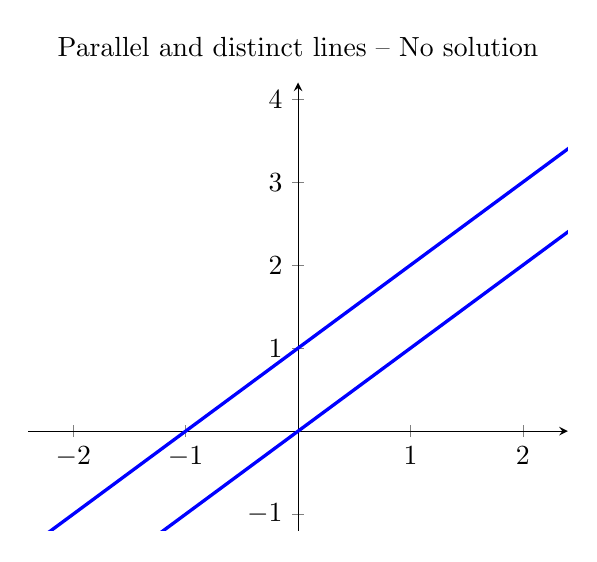
\begin{tikzpicture}
  \begin{axis}[
  title={Parallel and distinct lines -- No solution},
  xmin=-2.4,
  xmax=2.4,
  ymin=-1.2,
  ymax=4.2,
  axis lines=center,
  every axis y label/.style=
    {at=(current axis.above origin),anchor=south},
  every axis x label/.style=
    {at=(current axis.right of origin),anchor=west},
  ]
\addplot [very thick, blue, smooth, samples=100] {x+1};
\addplot [very thick, blue, smooth, samples=100] {x};
\end{axis}
\end{tikzpicture}
\end{image}
\begin{image}
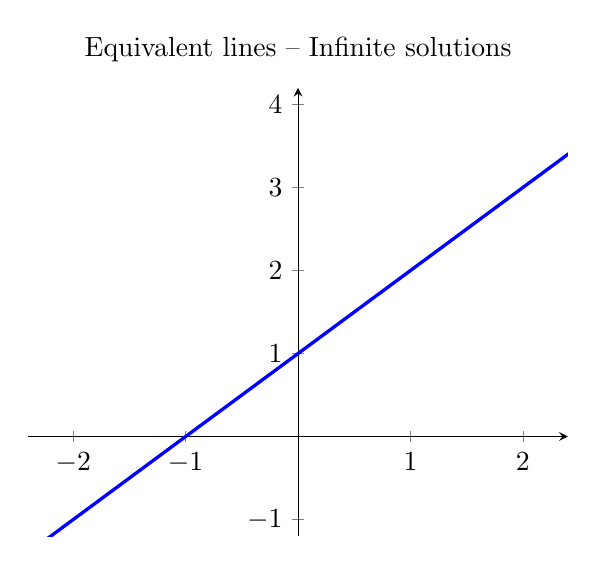
\begin{tikzpicture}
  \begin{axis}[
  title={Equivalent lines -- Infinite solutions},
  xmin=-2.4,
  xmax=2.4,
  ymin=-1.2,
  ymax=4.2,
  axis lines=center,
  every axis y label/.style=
    {at=(current axis.above origin),anchor=south},
  every axis x label/.style=
    {at=(current axis.right of origin),anchor=west},
  ]
\addplot [very thick, blue, smooth, samples=100] {x+1};
\end{axis}
\end{tikzpicture}
\end{image}